\documentclass[twoside]{book}

% Packages required by doxygen
\usepackage{fixltx2e}
\usepackage{calc}
\usepackage{doxygen}
\usepackage[export]{adjustbox} % also loads graphicx
\usepackage{graphicx}
\usepackage[utf8]{inputenc}
\usepackage{makeidx}
\usepackage{multicol}
\usepackage{multirow}
\PassOptionsToPackage{warn}{textcomp}
\usepackage{textcomp}
\usepackage[nointegrals]{wasysym}
\usepackage[table]{xcolor}

% Font selection
\usepackage[T1]{fontenc}
\usepackage[scaled=.90]{helvet}
\usepackage{courier}
\usepackage{amssymb}
\usepackage{sectsty}
\renewcommand{\familydefault}{\sfdefault}
\allsectionsfont{%
  \fontseries{bc}\selectfont%
  \color{darkgray}%
}
\renewcommand{\DoxyLabelFont}{%
  \fontseries{bc}\selectfont%
  \color{darkgray}%
}
\newcommand{\+}{\discretionary{\mbox{\scriptsize$\hookleftarrow$}}{}{}}

% Page & text layout
\usepackage{geometry}
\geometry{%
  a4paper,%
  top=2.5cm,%
  bottom=2.5cm,%
  left=2.5cm,%
  right=2.5cm%
}
\tolerance=750
\hfuzz=15pt
\hbadness=750
\setlength{\emergencystretch}{15pt}
\setlength{\parindent}{0cm}
\setlength{\parskip}{3ex plus 2ex minus 2ex}
\makeatletter
\renewcommand{\paragraph}{%
  \@startsection{paragraph}{4}{0ex}{-1.0ex}{1.0ex}{%
    \normalfont\normalsize\bfseries\SS@parafont%
  }%
}
\renewcommand{\subparagraph}{%
  \@startsection{subparagraph}{5}{0ex}{-1.0ex}{1.0ex}{%
    \normalfont\normalsize\bfseries\SS@subparafont%
  }%
}
\makeatother

% Headers & footers
\usepackage{fancyhdr}
\pagestyle{fancyplain}
\fancyhead[LE]{\fancyplain{}{\bfseries\thepage}}
\fancyhead[CE]{\fancyplain{}{}}
\fancyhead[RE]{\fancyplain{}{\bfseries\leftmark}}
\fancyhead[LO]{\fancyplain{}{\bfseries\rightmark}}
\fancyhead[CO]{\fancyplain{}{}}
\fancyhead[RO]{\fancyplain{}{\bfseries\thepage}}
\fancyfoot[LE]{\fancyplain{}{}}
\fancyfoot[CE]{\fancyplain{}{}}
\fancyfoot[RE]{\fancyplain{}{\bfseries\scriptsize Generated by Doxygen }}
\fancyfoot[LO]{\fancyplain{}{\bfseries\scriptsize Generated by Doxygen }}
\fancyfoot[CO]{\fancyplain{}{}}
\fancyfoot[RO]{\fancyplain{}{}}
\renewcommand{\footrulewidth}{0.4pt}
\renewcommand{\chaptermark}[1]{%
  \markboth{#1}{}%
}
\renewcommand{\sectionmark}[1]{%
  \markright{\thesection\ #1}%
}

% Indices & bibliography
\usepackage{natbib}
\usepackage[titles]{tocloft}
\setcounter{tocdepth}{3}
\setcounter{secnumdepth}{5}
\makeindex

% Hyperlinks (required, but should be loaded last)
\usepackage{ifpdf}
\ifpdf
  \usepackage[pdftex,pagebackref=true]{hyperref}
\else
  \usepackage[ps2pdf,pagebackref=true]{hyperref}
\fi
\hypersetup{%
  colorlinks=true,%
  linkcolor=blue,%
  citecolor=blue,%
  unicode%
}

% Custom commands
\newcommand{\clearemptydoublepage}{%
  \newpage{\pagestyle{empty}\cleardoublepage}%
}

\usepackage{caption}
\captionsetup{labelsep=space,justification=centering,font={bf},singlelinecheck=off,skip=4pt,position=top}

%===== C O N T E N T S =====

\begin{document}

% Titlepage & ToC
\hypersetup{pageanchor=false,
             bookmarksnumbered=true,
             pdfencoding=unicode
            }
\pagenumbering{roman}
\begin{titlepage}
\vspace*{7cm}
\begin{center}%
{\Large 3D Game Programming Assignment 1 \\[1ex]\large 1.\+2 }\\
\vspace*{1cm}
{\large Generated by Doxygen 1.8.11}\\
\end{center}
\end{titlepage}
\clearemptydoublepage
\tableofcontents
\clearemptydoublepage
\pagenumbering{arabic}
\hypersetup{pageanchor=true}

%--- Begin generated contents ---
\chapter{Hierarchical Index}
\section{Class Hierarchy}
This inheritance list is sorted roughly, but not completely, alphabetically\+:\begin{DoxyCompactList}
\item Frame\+Listener\begin{DoxyCompactList}
\item \contentsline{section}{Base\+Application}{\pageref{class_base_application}}{}
\begin{DoxyCompactList}
\item \contentsline{section}{Basic\+Tutorial\+\_\+00}{\pageref{class_basic_tutorial__00}}{}
\end{DoxyCompactList}
\end{DoxyCompactList}
\item Key\+Listener\begin{DoxyCompactList}
\item \contentsline{section}{Base\+Application}{\pageref{class_base_application}}{}
\end{DoxyCompactList}
\item Mouse\+Listener\begin{DoxyCompactList}
\item \contentsline{section}{Base\+Application}{\pageref{class_base_application}}{}
\end{DoxyCompactList}
\item Sdk\+Tray\+Listener\begin{DoxyCompactList}
\item \contentsline{section}{Base\+Application}{\pageref{class_base_application}}{}
\end{DoxyCompactList}
\item Window\+Event\+Listener\begin{DoxyCompactList}
\item \contentsline{section}{Base\+Application}{\pageref{class_base_application}}{}
\end{DoxyCompactList}
\end{DoxyCompactList}

\chapter{Class Index}
\section{Class List}
Here are the classes, structs, unions and interfaces with brief descriptions\+:\begin{DoxyCompactList}
\item\contentsline{section}{\hyperlink{class_base_application}{Base\+Application} }{\pageref{class_base_application}}{}
\item\contentsline{section}{\hyperlink{class_basic_tutorial__00}{Basic\+Tutorial\+\_\+00} \\*3D Game Programming ~\newline
My Name\+: Cliff Lee ~\newline
My ID\+: 0456620 ~\newline
My Email\+: \href{mailto:tommyboys0107@gmail.com}{\tt tommyboys0107@gmail.\+com} ~\newline
 Date\+: 2016/03/02 }{\pageref{class_basic_tutorial__00}}{}
\end{DoxyCompactList}

\chapter{Class Documentation}
\hypertarget{class_base_application}{}\section{Base\+Application Class Reference}
\label{class_base_application}\index{Base\+Application@{Base\+Application}}
Inheritance diagram for Base\+Application\+:\begin{figure}[H]
\begin{center}
\leavevmode
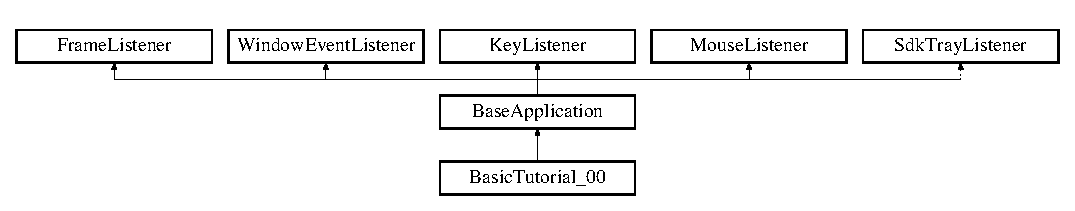
\includegraphics[height=2.382979cm]{class_base_application}
\end{center}
\end{figure}
\subsection*{Public Member Functions}
\begin{DoxyCompactItemize}
\item 
virtual void {\bfseries go} (void)\hypertarget{class_base_application_a8a14a65a29118dd75173aa68678a05e1}{}\label{class_base_application_a8a14a65a29118dd75173aa68678a05e1}

\end{DoxyCompactItemize}
\subsection*{Protected Member Functions}
\begin{DoxyCompactItemize}
\item 
virtual bool {\bfseries setup} ()\hypertarget{class_base_application_a5853d0e148cb85b0297a6885e1d33a89}{}\label{class_base_application_a5853d0e148cb85b0297a6885e1d33a89}

\item 
virtual bool {\bfseries configure} (void)\hypertarget{class_base_application_a62ed46f90e9f82cc810997647a2c587e}{}\label{class_base_application_a62ed46f90e9f82cc810997647a2c587e}

\item 
virtual void {\bfseries choose\+Scene\+Manager} (void)\hypertarget{class_base_application_ad5bc9655041e1849a4c13f444a3712bd}{}\label{class_base_application_ad5bc9655041e1849a4c13f444a3712bd}

\item 
virtual void {\bfseries create\+Camera} (void)\hypertarget{class_base_application_afa9d51527763cf9aee9cd4e1b1039d55}{}\label{class_base_application_afa9d51527763cf9aee9cd4e1b1039d55}

\item 
virtual void {\bfseries create\+Frame\+Listener} (void)\hypertarget{class_base_application_aff6fd9ff1ff0978cc68f19dd65be4778}{}\label{class_base_application_aff6fd9ff1ff0978cc68f19dd65be4778}

\item 
virtual void {\bfseries create\+Scene} (void)=0\hypertarget{class_base_application_aa97beeb4059b17d0ec22eae33286ec2d}{}\label{class_base_application_aa97beeb4059b17d0ec22eae33286ec2d}

\item 
virtual void {\bfseries destroy\+Scene} (void)\hypertarget{class_base_application_a365146059b25391fe400f5fdb94f011e}{}\label{class_base_application_a365146059b25391fe400f5fdb94f011e}

\item 
virtual void {\bfseries create\+Viewports} (void)\hypertarget{class_base_application_a1f8f6730cae6ec769d8730b1af48486e}{}\label{class_base_application_a1f8f6730cae6ec769d8730b1af48486e}

\item 
virtual void {\bfseries setup\+Resources} (void)\hypertarget{class_base_application_ae27301702f1e5de64619a39b1929f1f9}{}\label{class_base_application_ae27301702f1e5de64619a39b1929f1f9}

\item 
virtual void {\bfseries create\+Resource\+Listener} (void)\hypertarget{class_base_application_a9b77972f0f747a61e1f8ceba2ad47641}{}\label{class_base_application_a9b77972f0f747a61e1f8ceba2ad47641}

\item 
virtual void {\bfseries load\+Resources} (void)\hypertarget{class_base_application_aaeb764e637dd87601a81a80156659d88}{}\label{class_base_application_aaeb764e637dd87601a81a80156659d88}

\item 
virtual bool {\bfseries frame\+Rendering\+Queued} (const Ogre\+::\+Frame\+Event \&evt)\hypertarget{class_base_application_a03912a0f38b38fede7f08a2571e8fc56}{}\label{class_base_application_a03912a0f38b38fede7f08a2571e8fc56}

\item 
virtual bool {\bfseries key\+Pressed} (const O\+I\+S\+::\+Key\+Event \&arg)\hypertarget{class_base_application_acfa977f04e435f18018ece805c1277ec}{}\label{class_base_application_acfa977f04e435f18018ece805c1277ec}

\item 
virtual bool {\bfseries key\+Released} (const O\+I\+S\+::\+Key\+Event \&arg)\hypertarget{class_base_application_aba5c7c9dea7a0efc58b89310bae547e5}{}\label{class_base_application_aba5c7c9dea7a0efc58b89310bae547e5}

\item 
virtual bool {\bfseries mouse\+Moved} (const O\+I\+S\+::\+Mouse\+Event \&arg)\hypertarget{class_base_application_a126e59cb246b061e51eb6ce06a2ee8f4}{}\label{class_base_application_a126e59cb246b061e51eb6ce06a2ee8f4}

\item 
virtual bool {\bfseries mouse\+Pressed} (const O\+I\+S\+::\+Mouse\+Event \&arg, O\+I\+S\+::\+Mouse\+Button\+ID id)\hypertarget{class_base_application_a9255dfc1eabefd11c474ec45a6622504}{}\label{class_base_application_a9255dfc1eabefd11c474ec45a6622504}

\item 
virtual bool {\bfseries mouse\+Released} (const O\+I\+S\+::\+Mouse\+Event \&arg, O\+I\+S\+::\+Mouse\+Button\+ID id)\hypertarget{class_base_application_aa102c5859c14c0690c749994a446b53d}{}\label{class_base_application_aa102c5859c14c0690c749994a446b53d}

\item 
virtual void {\bfseries window\+Resized} (Ogre\+::\+Render\+Window $\ast$rw)\hypertarget{class_base_application_afacf8a797588592ef0abbad593f10cfa}{}\label{class_base_application_afacf8a797588592ef0abbad593f10cfa}

\item 
virtual void {\bfseries window\+Closed} (Ogre\+::\+Render\+Window $\ast$rw)\hypertarget{class_base_application_ae0e37ac54a31ff6e51d58c7654ad1b90}{}\label{class_base_application_ae0e37ac54a31ff6e51d58c7654ad1b90}

\end{DoxyCompactItemize}
\subsection*{Protected Attributes}
\begin{DoxyCompactItemize}
\item 
Ogre\+::\+Root $\ast$ {\bfseries m\+Root}\hypertarget{class_base_application_add84ba707dc6c57e6283f214b1274110}{}\label{class_base_application_add84ba707dc6c57e6283f214b1274110}

\item 
Ogre\+::\+Camera $\ast$ {\bfseries m\+Camera}\hypertarget{class_base_application_a3829c6b12afe911e97e6b4524b33a38b}{}\label{class_base_application_a3829c6b12afe911e97e6b4524b33a38b}

\item 
Ogre\+::\+Scene\+Manager $\ast$ {\bfseries m\+Scene\+Mgr}\hypertarget{class_base_application_a8a7684f4f9a57ed3089048ad1a913b2d}{}\label{class_base_application_a8a7684f4f9a57ed3089048ad1a913b2d}

\item 
Ogre\+::\+Render\+Window $\ast$ {\bfseries m\+Window}\hypertarget{class_base_application_ac5d8e9c81e036897bc82f81eff8c570f}{}\label{class_base_application_ac5d8e9c81e036897bc82f81eff8c570f}

\item 
Ogre\+::\+String {\bfseries m\+Resources\+Cfg}\hypertarget{class_base_application_a765e0df01c141a16df3178ab4f17afe6}{}\label{class_base_application_a765e0df01c141a16df3178ab4f17afe6}

\item 
Ogre\+::\+String {\bfseries m\+Plugins\+Cfg}\hypertarget{class_base_application_a04f2fe47fa164fd78d986dc0df70b7fb}{}\label{class_base_application_a04f2fe47fa164fd78d986dc0df70b7fb}

\item 
Ogre\+Bites\+::\+Sdk\+Tray\+Manager $\ast$ {\bfseries m\+Tray\+Mgr}\hypertarget{class_base_application_a7faa397f4f4861ee8c361a01e90b4416}{}\label{class_base_application_a7faa397f4f4861ee8c361a01e90b4416}

\item 
Ogre\+Bites\+::\+Sdk\+Camera\+Man $\ast$ {\bfseries m\+Camera\+Man}\hypertarget{class_base_application_a9ae38dea6316058549151fff66a91fcd}{}\label{class_base_application_a9ae38dea6316058549151fff66a91fcd}

\item 
Ogre\+Bites\+::\+Params\+Panel $\ast$ {\bfseries m\+Details\+Panel}\hypertarget{class_base_application_a6a11054ca61efdf558e0ff1b2de43a12}{}\label{class_base_application_a6a11054ca61efdf558e0ff1b2de43a12}

\item 
bool {\bfseries m\+Cursor\+Was\+Visible}\hypertarget{class_base_application_ac7e861799862cb645f1d78b170aef80d}{}\label{class_base_application_ac7e861799862cb645f1d78b170aef80d}

\item 
bool {\bfseries m\+Shut\+Down}\hypertarget{class_base_application_a755f26d3a9915aaf830750d877e39d86}{}\label{class_base_application_a755f26d3a9915aaf830750d877e39d86}

\item 
O\+I\+S\+::\+Input\+Manager $\ast$ {\bfseries m\+Input\+Manager}\hypertarget{class_base_application_abc9503c8462e225b5d0d55c952d9e4a9}{}\label{class_base_application_abc9503c8462e225b5d0d55c952d9e4a9}

\item 
O\+I\+S\+::\+Mouse $\ast$ {\bfseries m\+Mouse}\hypertarget{class_base_application_add9b97fbe64da2814d3af113bac58c43}{}\label{class_base_application_add9b97fbe64da2814d3af113bac58c43}

\item 
O\+I\+S\+::\+Keyboard $\ast$ {\bfseries m\+Keyboard}\hypertarget{class_base_application_a9d6e19cf50c47379fbaae55bff28079c}{}\label{class_base_application_a9d6e19cf50c47379fbaae55bff28079c}

\end{DoxyCompactItemize}


The documentation for this class was generated from the following files\+:\begin{DoxyCompactItemize}
\item 
Base\+Application.\+h\item 
Base\+Application.\+cpp\end{DoxyCompactItemize}

\hypertarget{class_basic_tutorial__00}{}\section{Basic\+Tutorial\+\_\+00 Class Reference}
\label{class_basic_tutorial__00}\index{Basic\+Tutorial\+\_\+00@{Basic\+Tutorial\+\_\+00}}


3D Game Programming ~\newline
My Name\+: Cliff Lee ~\newline
My ID\+: 0456620 ~\newline
My Email\+: \href{mailto:tommyboys0107@gmail.com}{\tt tommyboys0107@gmail.\+com} ~\newline
 Date\+: 2016/03/02  




{\ttfamily \#include $<$Tutorial\+Application.\+h$>$}

Inheritance diagram for Basic\+Tutorial\+\_\+00\+:\begin{figure}[H]
\begin{center}
\leavevmode
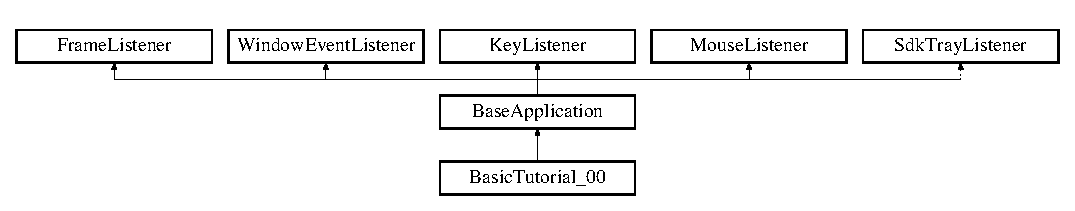
\includegraphics[height=2.382979cm]{class_basic_tutorial__00}
\end{center}
\end{figure}
\subsection*{Public Member Functions}
\begin{DoxyCompactItemize}
\item 
virtual void {\bfseries create\+Viewports} (void)\hypertarget{class_basic_tutorial__00_adc2454d9f8226e0958ecf702f355846e}{}\label{class_basic_tutorial__00_adc2454d9f8226e0958ecf702f355846e}

\item 
virtual void {\bfseries create\+Scene} (void)\hypertarget{class_basic_tutorial__00_a15a3d4673724ec99077ce992f996a550}{}\label{class_basic_tutorial__00_a15a3d4673724ec99077ce992f996a550}

\item 
virtual void {\bfseries create\+Camera} (void)\hypertarget{class_basic_tutorial__00_a1bf709417d654dffc2ea10987412b912}{}\label{class_basic_tutorial__00_a1bf709417d654dffc2ea10987412b912}

\item 
virtual void \hyperlink{class_basic_tutorial__00_aba97a29d983586d2dc8e108d3bccf721}{choose\+Scene\+Manager} (void)\hypertarget{class_basic_tutorial__00_aba97a29d983586d2dc8e108d3bccf721}{}\label{class_basic_tutorial__00_aba97a29d983586d2dc8e108d3bccf721}

\begin{DoxyCompactList}\small\item\em Create and assign scene manager. \end{DoxyCompactList}\end{DoxyCompactItemize}
\subsection*{Private Member Functions}
\begin{DoxyCompactItemize}
\item 
void \hyperlink{class_basic_tutorial__00_a6d4684502f2f7b2cf628a975d7750d8e}{create\+Viewport\+\_\+00} (void)\hypertarget{class_basic_tutorial__00_a6d4684502f2f7b2cf628a975d7750d8e}{}\label{class_basic_tutorial__00_a6d4684502f2f7b2cf628a975d7750d8e}

\begin{DoxyCompactList}\small\item\em Create viewprot for scene 0\textquotesingle{}s main camera, and it\textquotesingle{}s full screen. \end{DoxyCompactList}\item 
void \hyperlink{class_basic_tutorial__00_a2801a2f0d91d80b471da48344d2ccccf}{create\+Viewport\+\_\+01} (void)\hypertarget{class_basic_tutorial__00_a2801a2f0d91d80b471da48344d2ccccf}{}\label{class_basic_tutorial__00_a2801a2f0d91d80b471da48344d2ccccf}

\begin{DoxyCompactList}\small\item\em Create viewprot for scene 1\textquotesingle{}s main camera, and it\textquotesingle{}s on the upper right corner with 1/4 windows witdth and height. \end{DoxyCompactList}\item 
void \hyperlink{class_basic_tutorial__00_a3479c50dbf8dc06a7ea77014eb94c6e7}{create\+Camera\+\_\+00} ()\hypertarget{class_basic_tutorial__00_a3479c50dbf8dc06a7ea77014eb94c6e7}{}\label{class_basic_tutorial__00_a3479c50dbf8dc06a7ea77014eb94c6e7}

\begin{DoxyCompactList}\small\item\em Create camera for scene 1. \end{DoxyCompactList}\item 
void \hyperlink{class_basic_tutorial__00_a8745a127adeb69fa769f832fd41412c0}{create\+Camera\+\_\+01} ()\hypertarget{class_basic_tutorial__00_a8745a127adeb69fa769f832fd41412c0}{}\label{class_basic_tutorial__00_a8745a127adeb69fa769f832fd41412c0}

\begin{DoxyCompactList}\small\item\em Create camera for scene 0. \end{DoxyCompactList}\item 
void {\bfseries create\+Scene\+\_\+00} ()\hypertarget{class_basic_tutorial__00_aa84173e509858146cbfb98274c1ef56e}{}\label{class_basic_tutorial__00_aa84173e509858146cbfb98274c1ef56e}

\item 
void {\bfseries create\+Scene\+\_\+01} ()\hypertarget{class_basic_tutorial__00_aad14e1ca565797c4b7dcff31bc0e1494}{}\label{class_basic_tutorial__00_aad14e1ca565797c4b7dcff31bc0e1494}

\item 
void \hyperlink{class_basic_tutorial__00_adc00264bf47afe1b689c04d7e7ded79a}{Create\+Plane\+Mesh} ()\hypertarget{class_basic_tutorial__00_adc00264bf47afe1b689c04d7e7ded79a}{}\label{class_basic_tutorial__00_adc00264bf47afe1b689c04d7e7ded79a}

\begin{DoxyCompactList}\small\item\em Create plane mesh data. \end{DoxyCompactList}\item 
void \hyperlink{class_basic_tutorial__00_a85d22e164f65d875ed6e819316efb534}{Create\+First\+Cube\+Row} (Ogre\+::\+Scene\+Manager $\ast$scene\+Manager, Ogre\+::\+String row\+Name, int cube\+Num=30, float length=255.\+0f)
\begin{DoxyCompactList}\small\item\em Create needed first cube row. \end{DoxyCompactList}\item 
void \hyperlink{class_basic_tutorial__00_af24f6ce5c00cade7cabf19acdde8d45a}{Create\+Second\+Cube\+Row} (Ogre\+::\+Scene\+Manager $\ast$scene\+Manager, Ogre\+::\+String row\+Name, int cube\+Num=30, float length=255.\+0f)
\begin{DoxyCompactList}\small\item\em Create needed second cube row. \end{DoxyCompactList}\end{DoxyCompactItemize}
\subsection*{Private Attributes}
\begin{DoxyCompactItemize}
\item 
Ogre\+::\+Camera $\ast$ \hyperlink{class_basic_tutorial__00_af8d457d912286a98c0975c52d4faf910}{m\+Camera\+Arr} \mbox{[}8\mbox{]}\hypertarget{class_basic_tutorial__00_af8d457d912286a98c0975c52d4faf910}{}\label{class_basic_tutorial__00_af8d457d912286a98c0975c52d4faf910}

\begin{DoxyCompactList}\small\item\em Array of cameras. \end{DoxyCompactList}\item 
Ogre\+::\+Scene\+Manager $\ast$ \hyperlink{class_basic_tutorial__00_a603779b6087698c57b7989e16d8a9b93}{m\+Scene\+Mgr\+Arr} \mbox{[}8\mbox{]}\hypertarget{class_basic_tutorial__00_a603779b6087698c57b7989e16d8a9b93}{}\label{class_basic_tutorial__00_a603779b6087698c57b7989e16d8a9b93}

\begin{DoxyCompactList}\small\item\em Array of scene managers. \end{DoxyCompactList}\item 
Ogre\+Bites\+::\+Sdk\+Camera\+Man $\ast$ \hyperlink{class_basic_tutorial__00_a700c07f924c71e9fa1885a46f599d934}{m\+Camera\+Man\+Arr} \mbox{[}8\mbox{]}\hypertarget{class_basic_tutorial__00_a700c07f924c71e9fa1885a46f599d934}{}\label{class_basic_tutorial__00_a700c07f924c71e9fa1885a46f599d934}

\begin{DoxyCompactList}\small\item\em Array of camera controllers. \end{DoxyCompactList}\end{DoxyCompactItemize}
\subsection*{Additional Inherited Members}


\subsection{Detailed Description}
3D Game Programming ~\newline
My Name\+: Cliff Lee ~\newline
My ID\+: 0456620 ~\newline
My Email\+: \href{mailto:tommyboys0107@gmail.com}{\tt tommyboys0107@gmail.\+com} ~\newline
 Date\+: 2016/03/02 

This is an assignment of 3D Game Programming 

\subsection{Member Function Documentation}
\index{Basic\+Tutorial\+\_\+00@{Basic\+Tutorial\+\_\+00}!Create\+First\+Cube\+Row@{Create\+First\+Cube\+Row}}
\index{Create\+First\+Cube\+Row@{Create\+First\+Cube\+Row}!Basic\+Tutorial\+\_\+00@{Basic\+Tutorial\+\_\+00}}
\subsubsection[{\texorpdfstring{Create\+First\+Cube\+Row(\+Ogre\+::\+Scene\+Manager $\ast$scene\+Manager, Ogre\+::\+String row\+Name, int cube\+Num=30, float length=255.\+0f)}{CreateFirstCubeRow(Ogre::SceneManager *sceneManager, Ogre::String rowName, int cubeNum=30, float length=255.0f)}}]{\setlength{\rightskip}{0pt plus 5cm}void Basic\+Tutorial\+\_\+00\+::\+Create\+First\+Cube\+Row (
\begin{DoxyParamCaption}
\item[{Ogre\+::\+Scene\+Manager $\ast$}]{scene\+Manager, }
\item[{Ogre\+::\+String}]{row\+Name, }
\item[{int}]{cube\+Num = {\ttfamily 30}, }
\item[{float}]{length = {\ttfamily 255.0f}}
\end{DoxyParamCaption}
)\hspace{0.3cm}{\ttfamily [private]}}\hypertarget{class_basic_tutorial__00_a85d22e164f65d875ed6e819316efb534}{}\label{class_basic_tutorial__00_a85d22e164f65d875ed6e819316efb534}


Create needed first cube row. 

Create cube row with ~\newline
height = 50 $\ast$ (1 + cos(x $\ast$ 2 $\ast$ 3.\+1415), ~\newline
z = -\/125.\+0f.


\begin{DoxyParams}{Parameters}
{\em scene\+Manager} & Scene manager that you want to create cube row in. \\
\hline
{\em row\+Name} & Cube row name that will naming as follow \+: row\+Name0, row\+Name1, row\+Name2, ...etc. \\
\hline
{\em cube\+Num} & Determine how many cubes in the row. \\
\hline
{\em length} & Determine how long the row is. \\
\hline
\end{DoxyParams}
\begin{DoxySeeAlso}{See also}
\hyperlink{class_basic_tutorial__00_af24f6ce5c00cade7cabf19acdde8d45a}{Create\+Second\+Cube\+Row()} 
\end{DoxySeeAlso}
\index{Basic\+Tutorial\+\_\+00@{Basic\+Tutorial\+\_\+00}!Create\+Second\+Cube\+Row@{Create\+Second\+Cube\+Row}}
\index{Create\+Second\+Cube\+Row@{Create\+Second\+Cube\+Row}!Basic\+Tutorial\+\_\+00@{Basic\+Tutorial\+\_\+00}}
\subsubsection[{\texorpdfstring{Create\+Second\+Cube\+Row(\+Ogre\+::\+Scene\+Manager $\ast$scene\+Manager, Ogre\+::\+String row\+Name, int cube\+Num=30, float length=255.\+0f)}{CreateSecondCubeRow(Ogre::SceneManager *sceneManager, Ogre::String rowName, int cubeNum=30, float length=255.0f)}}]{\setlength{\rightskip}{0pt plus 5cm}void Basic\+Tutorial\+\_\+00\+::\+Create\+Second\+Cube\+Row (
\begin{DoxyParamCaption}
\item[{Ogre\+::\+Scene\+Manager $\ast$}]{scene\+Manager, }
\item[{Ogre\+::\+String}]{row\+Name, }
\item[{int}]{cube\+Num = {\ttfamily 30}, }
\item[{float}]{length = {\ttfamily 255.0f}}
\end{DoxyParamCaption}
)\hspace{0.3cm}{\ttfamily [private]}}\hypertarget{class_basic_tutorial__00_af24f6ce5c00cade7cabf19acdde8d45a}{}\label{class_basic_tutorial__00_af24f6ce5c00cade7cabf19acdde8d45a}


Create needed second cube row. 

Create cube row with ~\newline
height = 20 $\ast$ (1 + sin(x $\ast$ 2 $\ast$ 3.\+1415), ~\newline
z = 125.\+0f.


\begin{DoxyParams}{Parameters}
{\em scene\+Manager} & Scene manager that you want to create cube row in. \\
\hline
{\em row\+Name} & Cube row name that will naming as follow \+: row\+Name0, row\+Name1, row\+Name2, ...etc. \\
\hline
{\em cube\+Num} & Determine how many cubes in the row. \\
\hline
{\em length} & Determine how long the row is. \\
\hline
\end{DoxyParams}
\begin{DoxySeeAlso}{See also}
\hyperlink{class_basic_tutorial__00_a85d22e164f65d875ed6e819316efb534}{Create\+First\+Cube\+Row()} 
\end{DoxySeeAlso}


The documentation for this class was generated from the following files\+:\begin{DoxyCompactItemize}
\item 
Tutorial\+Application.\+h\item 
Tutorial\+Application.\+cpp\end{DoxyCompactItemize}

%--- End generated contents ---

% Index
\backmatter
\newpage
\phantomsection
\clearemptydoublepage
\addcontentsline{toc}{chapter}{Index}
\printindex

\end{document}
